% Minimal audience deck. The original detailed deck and notes remain unchanged.
% Use lapflow-10-minute-speaker-notes.md for the spoken explanation and timing.
% Compile twice with pdfLaTeX. No external assets required.
\documentclass[aspectratio=169,12pt]{beamer}
\usepackage{amsmath,booktabs,tikz}
\usetikzlibrary{arrows.meta,positioning}
\usetheme{default}
\definecolor{ink}{RGB}{32,48,61}
\definecolor{accent}{RGB}{0,104,112}
\definecolor{soft}{RGB}{239,244,246}
\setbeamercolor{structure}{fg=ink}
\setbeamercolor{frametitle}{fg=ink}
\setbeamertemplate{navigation symbols}{}
\setbeamertemplate{footline}{\hfill\scriptsize\color{gray}\insertframenumber/9\hspace{0.5cm}\vspace{0.2cm}}
\setbeamertemplate{itemize items}[circle]
\setlength{\tabcolsep}{9pt}
\tikzset{box/.style={draw=ink!45,rounded corners=2pt,fill=soft,align=center,
 minimum height=1.15cm,text width=2.65cm,font=\large},
 arr/.style={-{Latex[length=2.5mm]},thick,draw=ink},
 lab/.style={font=\small,color=gray}}
\title{Generating 3D turbulence}
\subtitle{A LapFlow baseline}
\author{\textit{Your name}}
\date{\textit{Lab meeting date}}
\begin{document}

% 0:00--0:20
\begin{frame}[plain]
 \titlepage
\end{frame}

% 0:20--1:00
\begin{frame}{The task}
 \begin{center}
 {\Large Generate a new $(u,v,w)$ snapshot}\[0.7cm]
 {\Huge $384\times384\times384$}\[0.8cm]
 {\large Same spatial statistics as the DNS?}
 \end{center}
 \vfill
 {\small\color{gray}Unconditional generation. No physical-time forecast.}
\end{frame}

% 1:00--2:20
\begin{frame}{Why compress?}
 \begin{columns}[c]
  \begin{column}{0.48\textwidth}
   \centering {\Huge 648 MiB}\\[0.3cm]
   One velocity volume
  \end{column}
  \begin{column}{0.48\textwidth}
   \centering {\Huge 27 GiB}\\[0.3cm]
   One full-grid feature tensor\\
   {\small 128 channels, FP32}
  \end{column}
 \end{columns}
 \vspace{1cm}
 \begin{center}
  {\large Small 3D autoencoder\quad +\quad tiled computation}
 \end{center}
 \vfill
 {\small\color{gray}Feature memory is illustrative, before gradients. Deterministic AE chosen initially; a 3D VAE is possible.}
\end{frame}

% 2:20--3:35
\begin{frame}{Encoder and decoder}
 \begin{center}
 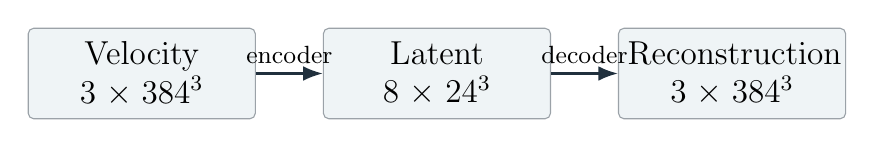
\begin{tikzpicture}[node distance=0.85cm]
  \node[box] (u) {Velocity\\$3\times384^3$};
  \node[box,right=of u] (z) {Latent\\$8\times24^3$};
  \node[box,right=of z] (r) {Reconstruction\\$3\times384^3$};
  \draw[arr] (u)--node[above,font=\small]{encoder} (z);
  \draw[arr] (z)--node[above,font=\small]{decoder} (r);
 \end{tikzpicture}
 \end{center}
 \vspace{0.4cm}
 \[
 L_{\mathrm{AE}}=\operatorname{MSE}\!\left(D(E(\widetilde U)),\widetilde U\right)
 \]
 \begin{center}
 {\small Four stride-2 convolutions: $384\to192\to96\to48\to24$}\\[0.2cm]
 {\small Encoder: 35,552 parameters}\[0.45cm]
 {\large Train together. Freeze before flow training.}
 \end{center}
 \vfill
 {\footnotesize\color{gray}MSE is scored on the crop core. Latent channels are learned features.}
\end{frame}

% 3:35--4:50
\begin{frame}{What survives compression?}
 \begin{center}
 {\Huge $1536\times$}\[0.25cm]
 {\large fewer scalar values}\[0.7cm]
 \end{center}
 \begin{columns}[T]
  \begin{column}{0.48\textwidth}
   \centering \textbf{Risk}\\[0.25cm]
   Lost fine detail\\
   Smoothed fluctuations
  \end{column}
  \begin{column}{0.48\textwidth}
   \centering \textbf{Check first}\\[0.25cm]
   Reconstruction spectrum\\
   Reconstruction energy
  \end{column}
 \end{columns}
 \vfill
 \begin{center}
 {\large A $384^3$ output does not guarantee DNS fidelity.}
 \end{center}
\end{frame}

% 4:50--6:10
\begin{frame}{The Laplacian pyramid}
 \begin{center}
 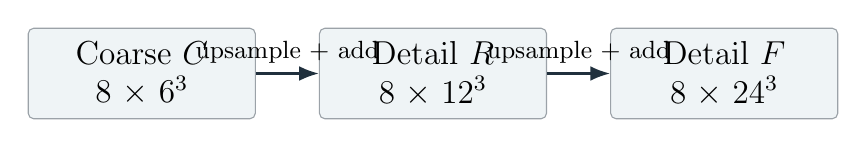
\begin{tikzpicture}[node distance=0.8cm]
  \node[box] (c) {Coarse $C$\\$8\times6^3$};
  \node[box,right=of c] (r) {Detail $R$\\$8\times12^3$};
  \node[box,right=of r] (f) {Detail $F$\\$8\times24^3$};
  \draw[arr] (c)--node[above,font=\small]{upsample + add} (r);
  \draw[arr] (r)--node[above,font=\small]{upsample + add} (f);
 \end{tikzpicture}
 \end{center}
 \vspace{0.3cm}
 \[
 \begin{aligned}
  C&=P(P(Z)), & R&=P(Z)-A(C), & F&=Z-A(P(Z))
 \end{aligned}
 \]
 \[
 \boxed{Z=A\bigl(A(C)+R\bigr)+F}
 \]
 \vfill
 {\small $P$: average pooling.\quad $A$: nearest-neighbor upsampling.}\\[0.2cm]
 {\small\color{gray}Exact latent reconstruction. These are not physical Fourier bands.}
\end{frame}

% 6:10--7:30
\begin{frame}{Learning the flow}
 \begin{columns}[c]
  \begin{column}{0.57\textwidth}
   \[
   \begin{aligned}
    \dot x_C&=v_C(x_C,\tau)\\[0.2cm]
    \dot x_R&=v_R(x_C,x_R,\tau)\\[0.2cm]
    \dot x_F&=v_F(x_C,x_R,x_F,\tau)
   \end{aligned}
   \]
  \end{column}
  \begin{column}{0.39\textwidth}
   \textbf{Attention context}\\[0.3cm]
   Coarse sees coarse.\\[0.2cm]
   Middle sees both.\\[0.2cm]
   Fine sees all three.
  \end{column}
 \end{columns}
 \vspace{0.45cm}
 \[
 L_{\mathrm{flow}}=L_C+L_R+L_F\qquad\text{(active bands)}
 \]
 \begin{center}
 {\large Separate outputs. One coupled training objective.}
 \end{center}
 \vfill
 {\small\color{gray}$\tau$ is generation time. Velocity is transport in latent space.}
\end{frame}

% 7:30--8:30
\begin{frame}{From noise to a field}
 \begin{center}
 \begin{tabular}{lll}
 \toprule
 $0\to1/3$ & $1/3\to2/3$ & $2/3\to1$\\
 \midrule
 Coarse & Coarse + middle & All three\\
 \bottomrule
 \end{tabular}
 \end{center}
 \vspace{0.6cm}
 \begin{center}
 {\Large Coarse states keep evolving.}\\[0.6cm]
 {\large Recombine bands $\;\to\;$ decode $\;\to\;$ velocity}
 \end{center}
 \vfill
 {\small\color{gray}48 Heun steps; 96 model evaluations. Random seeds give different samples.}
\end{frame}

% 8:30--10:00
\begin{frame}{What do we need to measure?}
 \begin{columns}[T]
  \begin{column}{0.48\textwidth}
   \textbf{Compression}\\[0.35cm]
   DNS versus its reconstruction\\[0.4cm]
   Spectrum\\
   Energy\\
   Pointwise error
  \end{column}
  \begin{column}{0.48\textwidth}
   \textbf{Generation}\\[0.35cm]
   Generated versus held-out DNS\\[0.4cm]
   Spectrum and energy\\
   Velocity PDFs\\
   Divergence and diversity
  \end{column}
 \end{columns}
 \vfill
 {\small\color{gray}Full-resolution GPU pipeline test passed. Learned quality remains to be evaluated.}\\[0.2cm]
 {\footnotesize\color{gray}3D adaptation of Zhao et al., LapFlow (2026): \url{https://arxiv.org/abs/2602.19461}}
\end{frame}

\end{document}
